\documentclass{article}
    \title{\textbf{Allegato1: Analisi app simili}}
	\date{}
	\usepackage{graphicx}
\begin{document}

\maketitle
\tableofcontents
\newpage

\section{Trivia Crack: Gioco a Quiz}
Si tratta di un gioco a quiz. Per poter usufruire dell’applicazione è necessaria una registrazione (mediante email o facendo login mediante un social network come Facebook). Una volta creato un account è possibile sfidare altre persone: possiamo scegliere un avversario che conosciamo oppure uno scelto in maniera aleatoria. Ad esempio, se colleghiamo il nostro account di Facebook, è possibile sfidare tutti gli amici che utilizzano all’applicazione. Una volta scelto un avversario inizia il gioco quindi viene scelta una categoria di domande (con un meccanismo simile ad una ruota della fortuna), e vengono visualizzate le domande a cui bisogna rispondere.

\subsection{Pro}
Un punto di forza di questa applicazione è sicuramente la componente social, in particolare:
\begin{itemize}
\item E’ presente una chat interna che permette di scambiare messaggi tra i vari giocatori avversari;
\item E’ possibile aggiungere degli amici (oltre a quelli di Facebook) in modo da potervi giocare più avanti senza doversi ricordare il nome utente;
\item E’ possibile creare nuove domande e modificare e dare un punteggio a quelle esistenti;
\item Presenza di una classifica con la quale è possibile confrontare il proprio punteggio con quello degli altri giocatori.
\end{itemize}

\subsection{Contro}
Di contro, è possibile evidenziare alcuni difetti:
\begin{itemize}
\item Troppi elementi nella schermata principale, è difficile orientarsi e non si capisce bene quale sia l’utilità di alcuni bottoni;
\item Troppe pubblicità invasive che appaiono in ogni schermata e in pop-up improvvisi;
\item Agli Utenti che non collegano il loro profilo con quello di Facebook viene assegnata una stringa come nickname (si veda l’ultima immagine).
\end{itemize}

\begin{figure}[htp]
\begin{center}
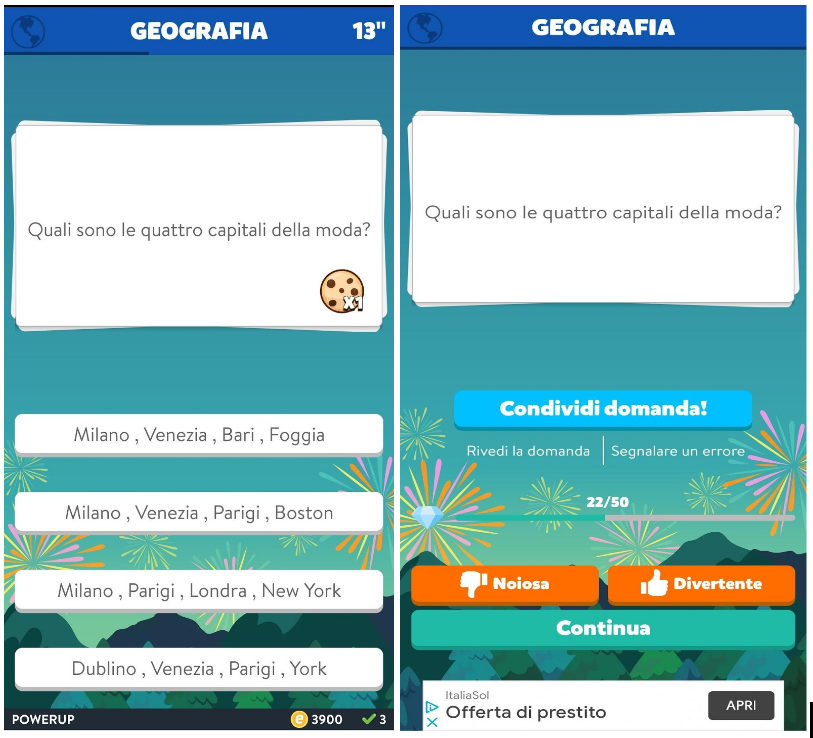
\includegraphics[width=1 \textwidth]{Figure1.png}
\caption{Trivia Crack - Interfaccia delle domande e resoconto risposta}
\end{center}
\end{figure}

\begin{figure}[htp]
\begin{center}
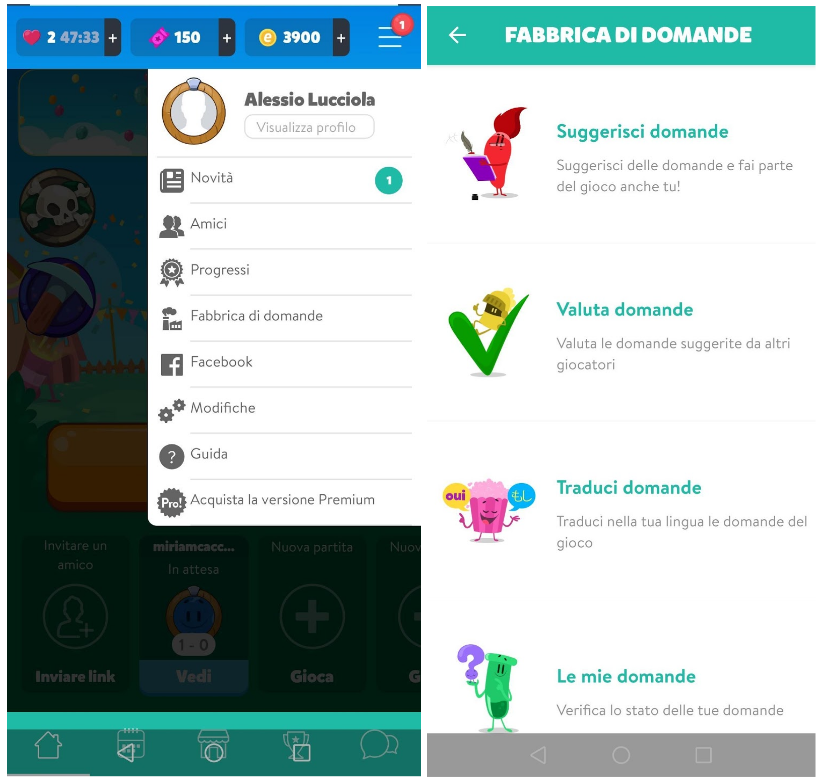
\includegraphics[width=1 \textwidth]{Figure2.png}
\caption{Trivia Crack - Creazione di domande personalizzate}
\end{center}
\end{figure}

\begin{figure}[htp]
\begin{center}
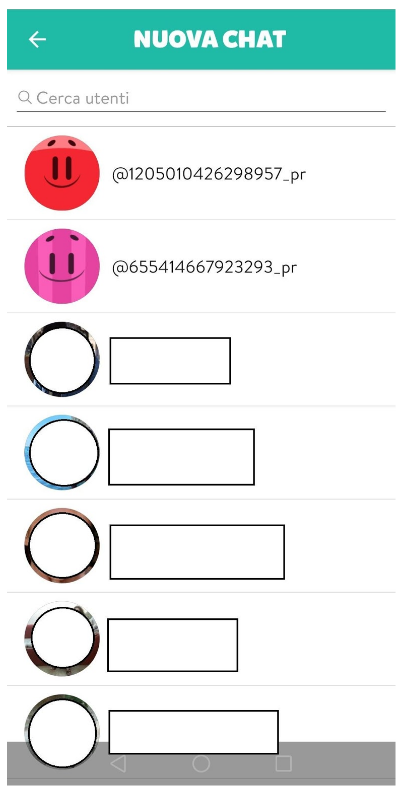
\includegraphics[width=0.5 \textwidth]{Figure3.png}
\caption{Trivia Crack - Chat in-game}
\end{center}
\end{figure}

\newpage

\section{LiveQuiz}
Si tratta di un gioco a quiz con vincite reali. Al contrario della altre applicazioni analizzate, LiveQuiz permette di giocare solamente in determinati orari e giorni stabiliti dal gioco. Ogni sessione di domande è incentrata su una categoria e tutti giocano allo stesso momento. Ogni giocatore possiede un punteggio che viene azzerato ogni lunedì. Ad ogni risposta corretta si ottengono dei punti che andranno a sommarsi alla punteggio settimanale. La domenica, le persone con il punteggio più alto nella classifica generale vincono dei premi (in denaro).

\subsection{Pro}
Alcuni aspetti positivi sono:
\begin{itemize}
\item Interfaccia semplice e lineare, tutto il necessario si trova in una sola schermata;
\item Possibilità di visionare il punteggio degli amici di Facebook che utilizzano il gioco;
\item Premi che spingono l'utente a giocare e a partecipare ad ogni evento;
\item Dopo aver visualizzato l’esito di ogni domanda, viene visualizzata una finestra con alcune curiosità relative alla domanda.
\end{itemize}

\subsection{Contro}
Alcuni aspetti negativi sono:
\begin{itemize}
\item Le domande sono spesso complesse e non di cultura generale;
\item La sola possibilità di giocare live.
\end{itemize}

\begin{figure}[htp]
\begin{center}
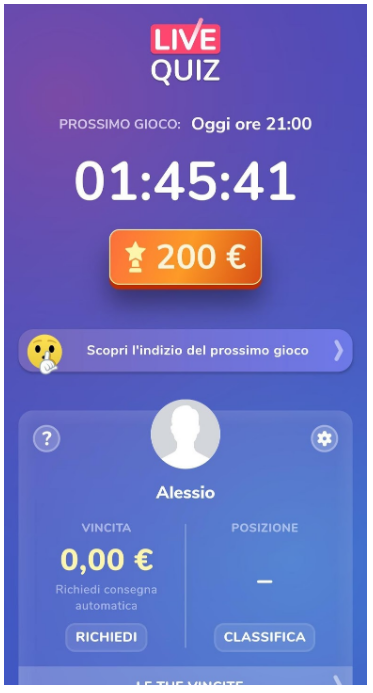
\includegraphics[width=0.5 \textwidth]{Figure4.png}
\caption{LiveQuiz - Schermata principale in cui si evidenzia il denaro guadagnato, ora e giorno del prossimo quiz, il punteggio ed il posto in classifica.
}
\end{center}
\end{figure}

\begin{figure}[htp]
\begin{center}
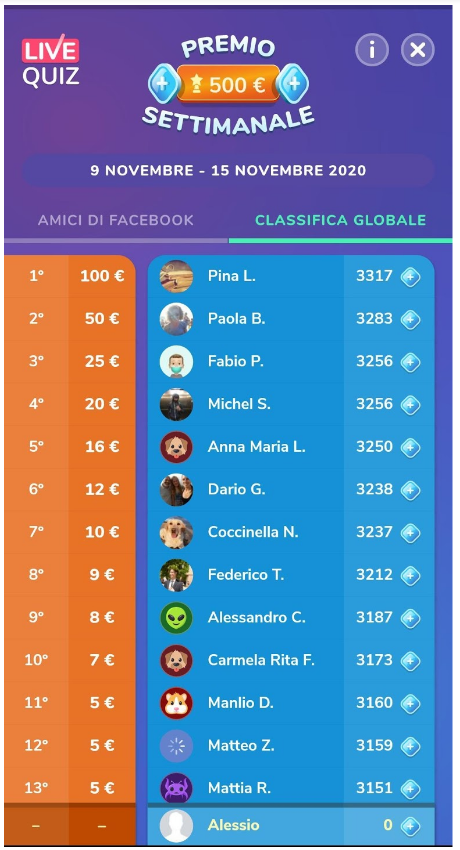
\includegraphics[width=0.5 \textwidth]{Figure5.png}
\caption{LiveQuiz - Classifica generale}
\end{center}
\end{figure}

\begin{figure}[htp]
\begin{center}
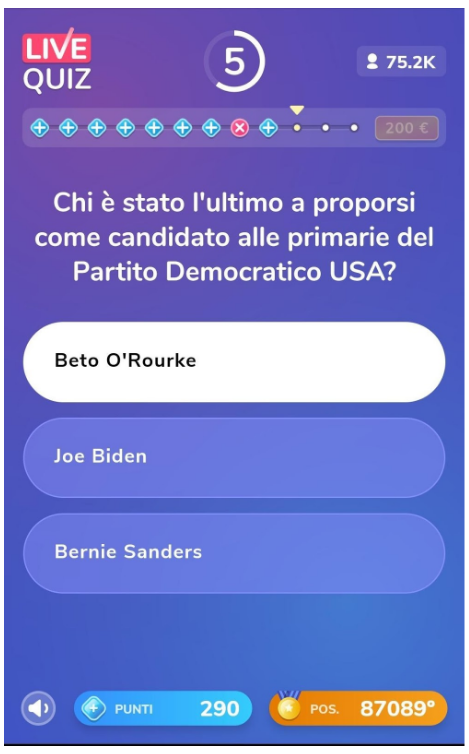
\includegraphics[width=0.5 \textwidth]{Figure6.png}
\caption{LiveQuiz - Struttura delle domande}
\end{center}
\end{figure}

\begin{figure}[htp]
\begin{center}
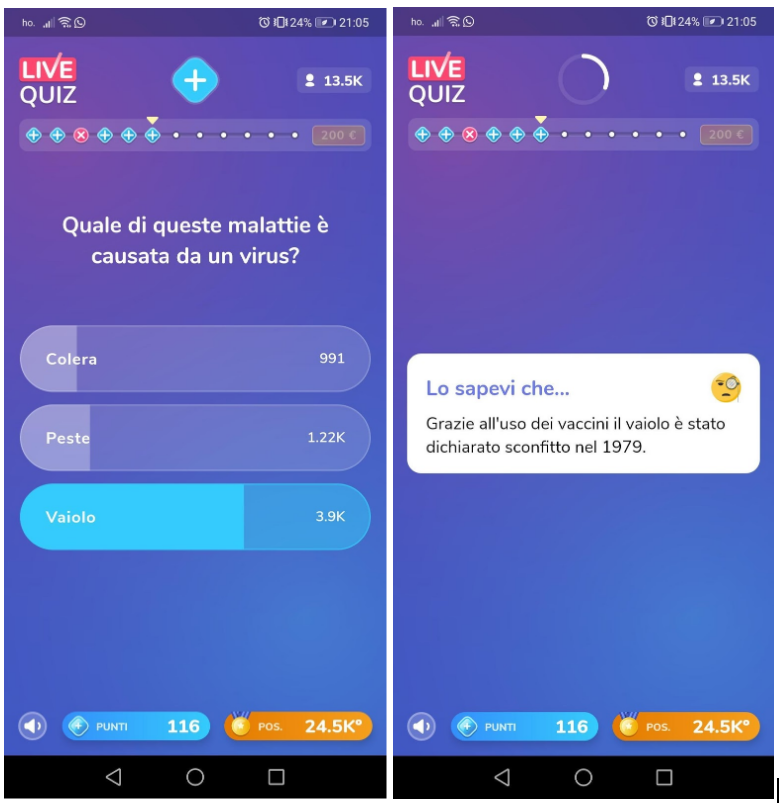
\includegraphics[width=1 \textwidth]{Figure7.png}
\caption{LiveQuiz - Interfaccia in seguito ad una risposta ed info}
\end{center}
\end{figure}


\newpage

\section{Quiz senza fine}
L’app ha un’interfaccia semplice ed intuitiva, appena si entra nell’applicazione si comincia subito a giocare trovandosi davanti subito una domanda. Il quiz consiste nel rispondere alle domande di qualsiasi ambito, si hanno quattro scelte di cui solo una giusta.
\\\indent
Cliccando il tasto in alto a sinistra si ha la possibilità di collegarsi al Google Play Giochi, il tasto “partita” permette di giocare le partite contro degli avversari casuali in cui c’è un limite di tempo per rispondere alla domanda, alla prima partita chiede di inserire un nome univoco, il tasto “imparare” rimanda ad una pagina Wikipedia della domanda precedente,  infine l’ultimo tasto rappresenta l’Elo del giocatore (ovvero un punteggio in base alle risposte giuste o sbagliate) e la lista delle domande a cui si ha risposto con la soluzione e la possibilità di andare a vedere su wikipedia.

\subsection{Pro}
Alcuni aspetti positivi:
\begin{itemize}
\item Interfaccia minimale e semplice;
\item Possibilità di giocare subito;
\item Rimandi a wikipedia per saperne di più sull’argomento.
\end{itemize}

\subsection{Contro}
Alcuni aspetti negativi:
\begin{itemize}
\item Poca integrazione con i social.
\end{itemize}

\begin{figure}[htp]
\begin{center}
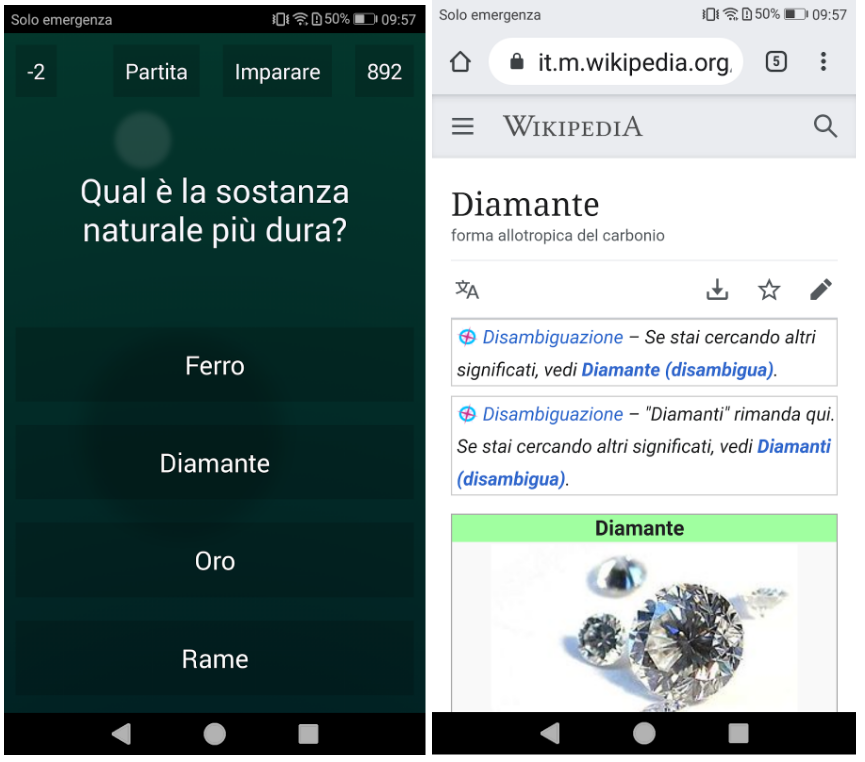
\includegraphics[width=1 \textwidth]{Figure8.png}
\caption{Quiz senza fine - Esempio di schermata con rimando a Wikipedia}
\end{center}
\end{figure}

\begin{figure}[htp]
\begin{center}
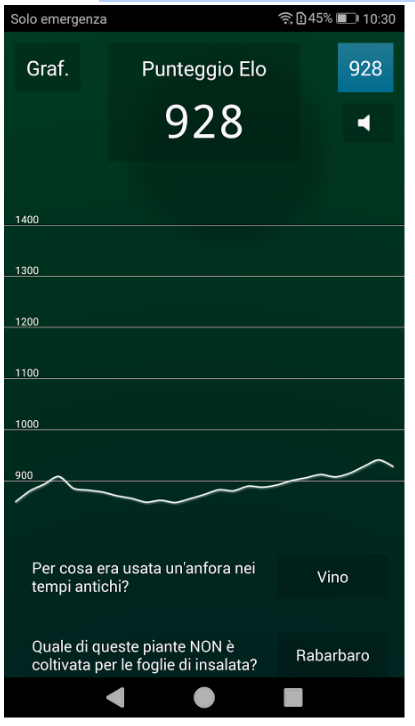
\includegraphics[width=0.5 \textwidth]{Figure9.png}
\caption{Quiz senza fine - Schermata Elo ed elenco delle domande}
\end{center}
\end{figure}

\begin{figure}[htp]
\begin{center}
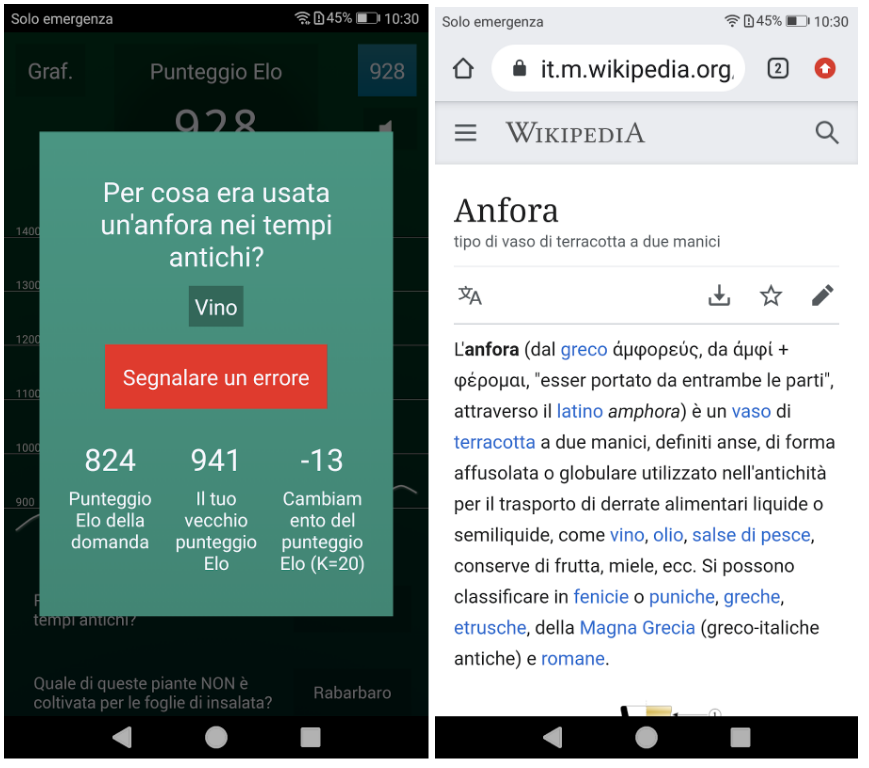
\includegraphics[width=1 \textwidth]{Figure10.png}
\caption{Quiz senza fine - Informazioni sulla domanda con possibilità di segnalare errori e di andare su Wikipedia}
\end{center}
\end{figure}

\newpage

\section{ArtQ!}
Si tratta di un gioco a quiz incentrato sull’arte. Il gioco prevede, prima di tutto, la creazione di un account (si può fare mediante email o utilizzando un account Google già esistente). Sulla schermata principale troviamo varie modalità di gioco quali:
\begin{itemize}
\item Flash Mode: Rispondi a più domande possibili (scelte casualmente) fino allo scadere del tempo;
\item Solo Mode: Quiz su varie categorie di domande divise per:
\begin{itemize}
\item Tipologia: Artisti, Dipinti, Periodo storico, Musei, etc..;
\item Movimento Artistico: Rinascimento, Barocco, Romanticismo, etc..;
\item Altre Categorie Specifiche: Street Art, Ritratti, etc..;
\end{itemize}
\item Multiplayer Mode: Sfida altri avversari (amici o scelti online casualmente).
\end{itemize}
Una volta scelta una categoria, la struttura del quiz è piuttosto semplice: viene posta una domande oppure viene mostrata una immagine e bisogna scegliere una della quattro possibili risposte.

\subsection{Pro}
Alcuni aspetti positivi dell’applicazione sono:
\begin{itemize}
\item Interfaccia di semplice utilizzo;
\item Possibilità di creare match personalizzati. In particolare, si può scegliere in numero di round e la difficoltà delle domande;
\item Giocando si sbloccano categorie sempre più difficili e con nuove domande (altrimenti si possono sbloccare direttamente con una valuta in-game, acquistabile con denaro reale).
\end{itemize}

\subsection{Contro}
Gli aspetti negativi sono:
\begin{itemize}
\item Scelte stilistiche dell’interfaccia a volte discutibili;
\item Componente social ridotta al minimo. La creazione dell’account è pressoché inutile in quanto non offre alcun particolare vantaggio all’interno dell’applicazione;
\item L’invito al match tramite email può essere scomodo.
\end{itemize}

\begin{figure}[htp]
\begin{center}
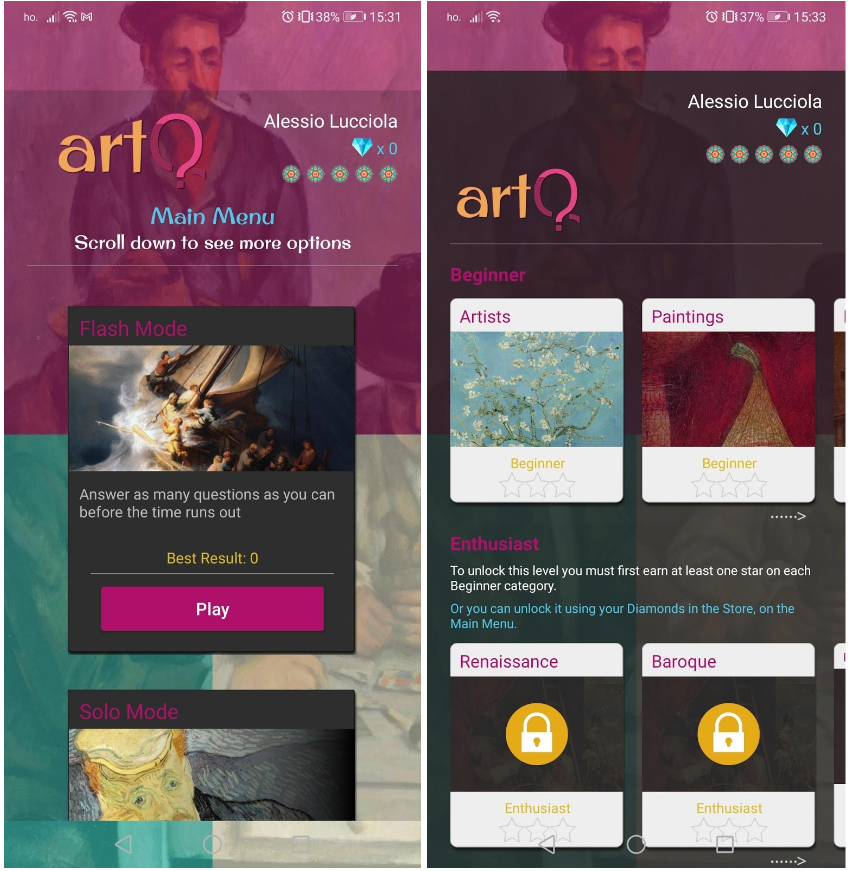
\includegraphics[width=1 \textwidth]{Figure11.png}
\caption{ArtQ! - Schermata principale e categorie domande}
\end{center}
\end{figure}

\begin{figure}[htp]
\begin{center}
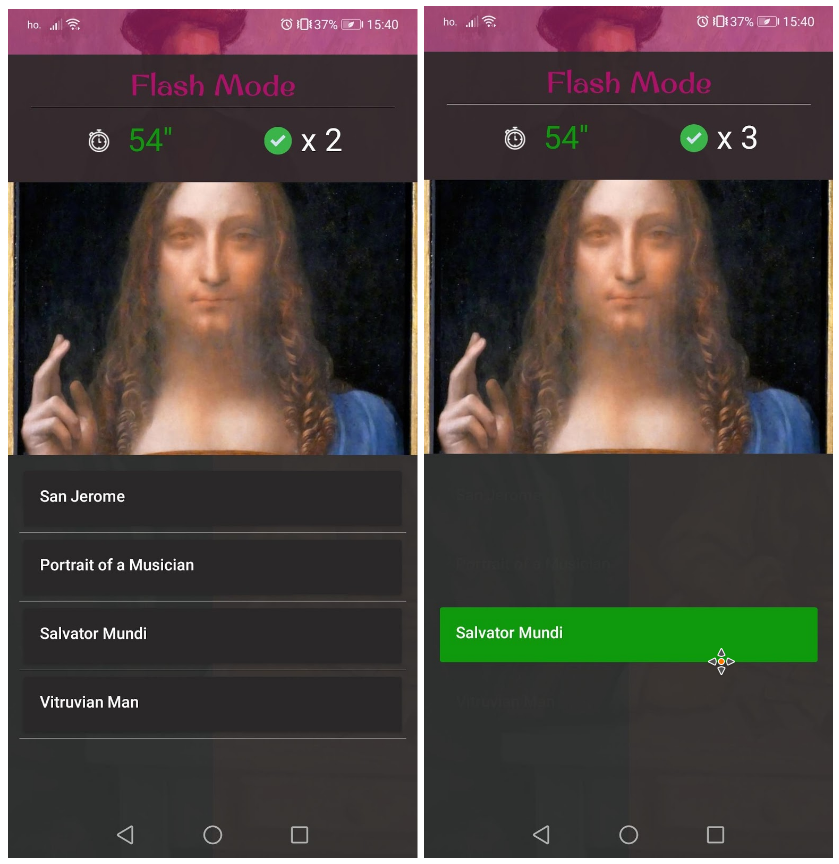
\includegraphics[width=1 \textwidth]{Figure12.png}
\caption{ArtQ! - Struttura delle domande}
\end{center}
\end{figure}

\begin{figure}[htp]
\begin{center}
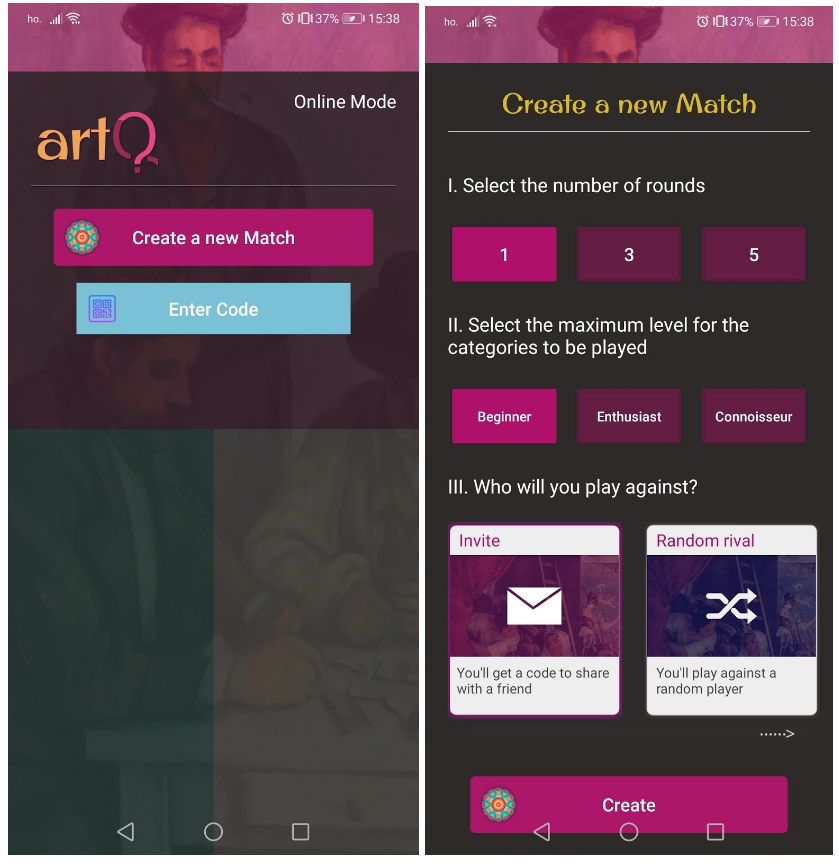
\includegraphics[width=1 \textwidth]{Figure13.png}
\caption{ArtQ! - Creazione di un match per il multigiocatore}
\end{center}
\end{figure}

\newpage

\section{Quiz d’arte in Italiano}
L’app consiste in un gioco a Quiz a tema arte. Ci sono tre tipologie di domande a cui bisogna rispondere entro un certo numero di secondi, quelle a scelta multipla, quelle in cui vengono date delle lettere tramite cui comporre la risposta ed infine quelle in cui bisogna rispondere vero o falso. Se non si riesce a rispondere alla domanda si può saltare oppure chiedere suggerimenti (che sono in numero limitato) o chiedere aiuto ad un amico condividendo la domanda tramite social, dopo aver risposto alla domanda verrà mostrata una curiosità inerente.
\\\indent
Nel gioco sono presenti delle vite che si ottengono entrando quotidianamente nell’app oppure comprandole o condividendo l'applicazione sui social, le vite si perdono quando non si riesce a rispondere correttamente alla domanda.

\subsection{Pro}
Alcuni aspetti positivi sono:
\begin{itemize}
\item Varie tipologie di risposta;
\item Possibilità di avere suggerimenti;
\item Curiosità inerenti;
\item Ottima componente social.
\end{itemize}

\subsection{Contro}
Alcuni aspetti negativi sono:
\begin{itemize}
\item pubblicità veramente troppo invasiva.
\end{itemize}

\begin{figure}[htp]
\begin{center}
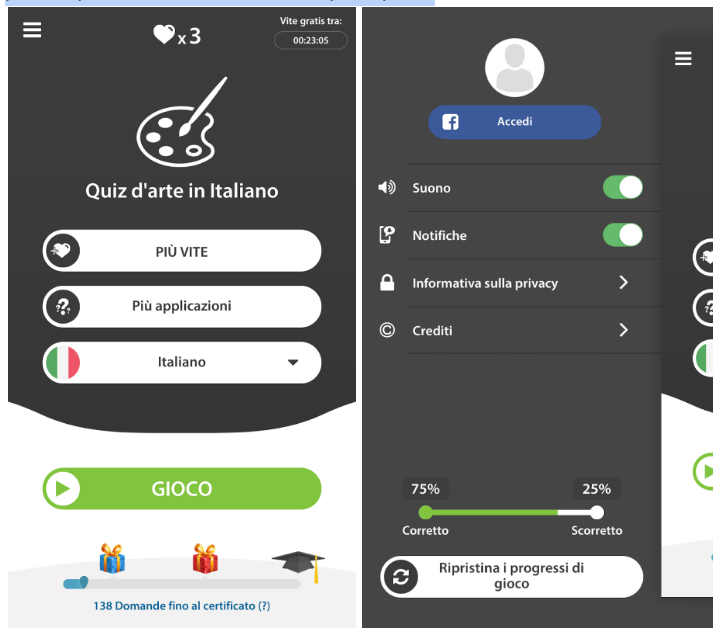
\includegraphics[width=1 \textwidth]{Figure14.png}
\caption{Quiz d’arte in Italiano - Schermata principale dell’applicazione e menù raggiungibile tramite pulsante a panino presente sulla schermata principale}
\end{center}
\end{figure}

\begin{figure}[htp]
\begin{center}
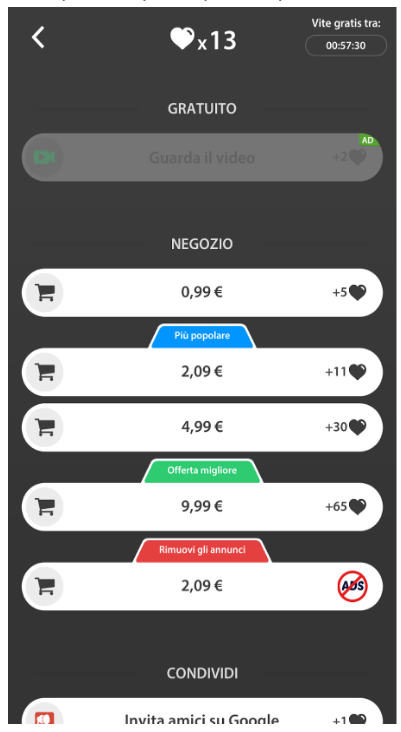
\includegraphics[width=0.5 \textwidth]{Figure15.png}
\caption{Quiz d’arte in Italiano - Shop dal quale si possono comprare vite}
\end{center}
\end{figure}

\begin{figure}[htp]
\begin{center}
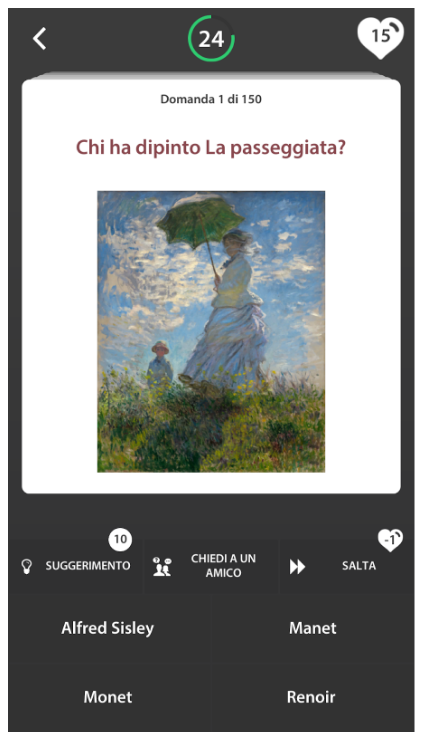
\includegraphics[width=0.5 \textwidth]{Figure16.png}
\caption{Quiz d’arte in Italiano - Domanda a risposta multipla. Si possono notare i suggerimenti, la condivisione ad un amico e la possibilità di saltare la domanda perdendo una vita}
\end{center}
\end{figure}

\begin{figure}[htp]
\begin{center}
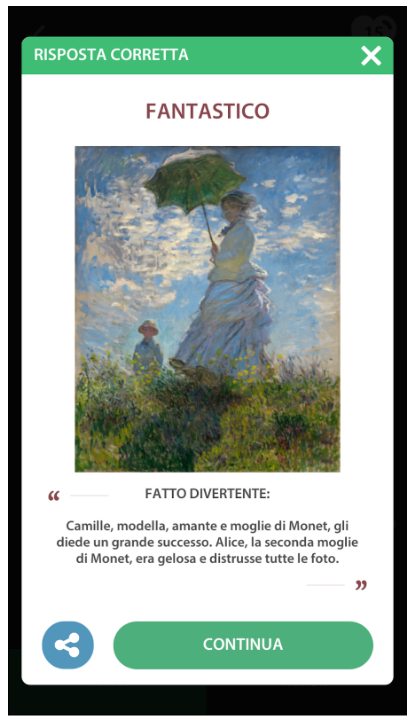
\includegraphics[width=0.5 \textwidth]{Figure17.png}
\caption{Quiz d’arte in Italiano - Curiosità in seguito ad una risposta}
\end{center}
\end{figure}

\begin{figure}[htp]
\begin{center}
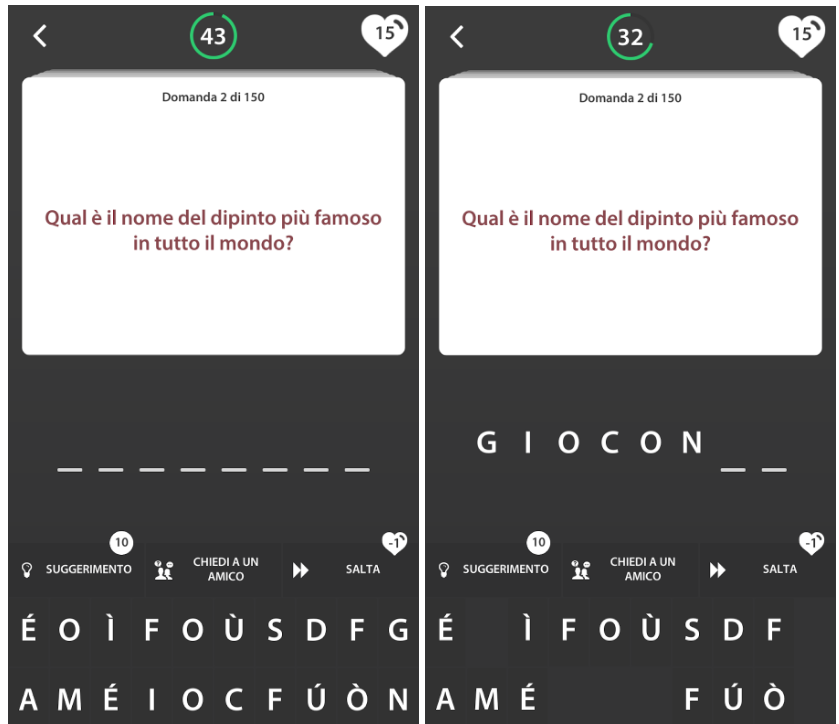
\includegraphics[width=1 \textwidth]{Figure18.png}
\caption{Quiz d’arte in Italiano - Altra tipologie di domande (in questo caso una risposta aperta e una domanda con opzione di risposta vero/falso)}
\end{center}
\end{figure}

\begin{figure}[htp]
\begin{center}
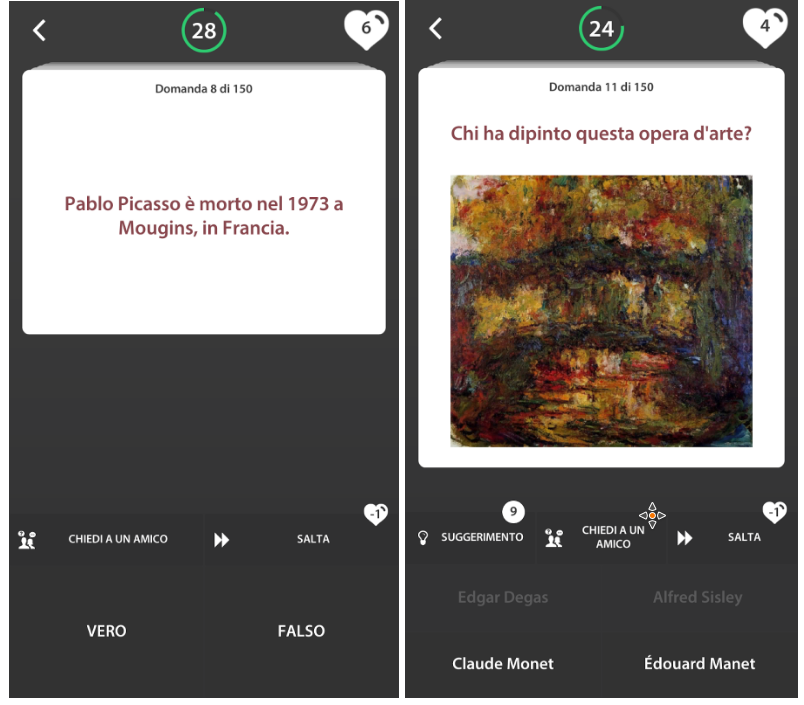
\includegraphics[width=1 \textwidth]{Figure19.png}
\caption{Quiz d’arte in Italiano - Funzionalità di suggerimento}
\end{center}
\end{figure}

\begin{figure}[htp]
\begin{center}
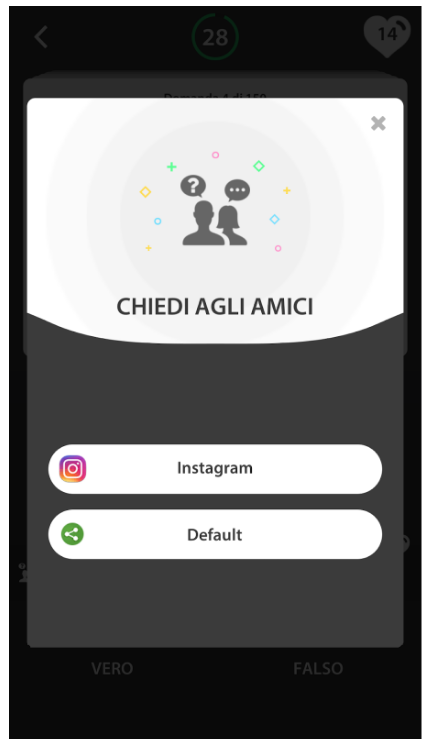
\includegraphics[width=0.5 \textwidth]{Figure20.png}
\caption{Quiz d’arte in Italiano - Schermata “chiedi agli amici” raggiungibile dalla precedente schermata}
\end{center}
\end{figure}

\newpage

\section{QuizDuello}
Si tratta di un gioco a quiz di cultura generale. Il gioco prevede la creazione di un account mediante email (è anche possibile giocare come ospite ed in tal caso verrà assegnato un nickname casuale). Una volta entrati nella schermata principale, è possibile avviare una nuova partita. Si può giocare con avversari casuali oppure effettuare il login su facebook e sfidare i propri conoscenti. Una volta scelto uno sfidante, si gioca: è possibile scegliere una delle categorie mostrate dal gioco e si dovrà rispondere a 3 domande. Ogni risposta corretta vale un punto. Dopo aver risposto alle 3 domande, si passa il turno all'avversario e così via per 6 turni. Alla fine vince chi ha totalizzato più punti.
\\\indent
Da rimarcare il fatto che è presente un’area “Arena” in cui vengono visualizzati eventi in corso: una volta selezionato un vento, vi si può partecipare utilizzando un biglietto (i biglietti si possono acquistare con denaro reale o facendo degli accessi giornalieri), quindi si sfideranno altri 4 giocatori. Vengono poste 6 domande, ad ogni risposta giusta si accumulano punti, alla fine vince la partita chi ha il punteggio più alto e la somma dei punti totalizzati andrà a sommarsi a quelli della classifica generale. Alla fine dell’evento, chi totalizza più punti nella classifica generale vince degli biglietti.

\subsection{Pro}
Gli aspetti positivi sono:
\begin{itemize}
\item Interfaccia minimale e semplice da utilizzare;
\item Possibilità di giocare con gli amici di Facebook;
\item Funzione Arena che permette di sfidare in diretta altri giocatori.
\end{itemize}

\subsection{Contro}
Non si evidenziano particolari aspetti negativi.

\begin{figure}[htp]
\begin{center}
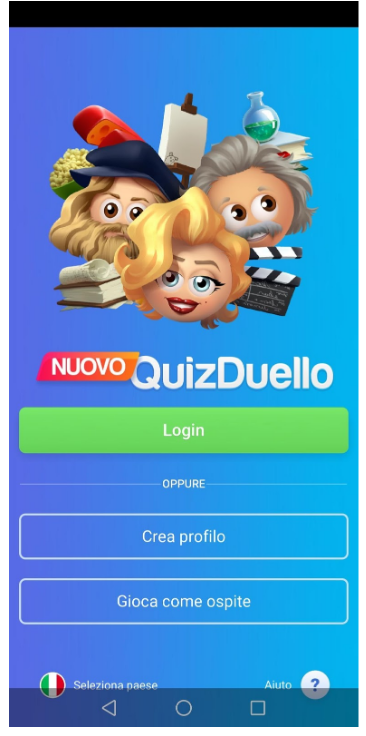
\includegraphics[width=0.5 \textwidth]{Figure21.png}
\caption{QuizDuello - Pagina di login}
\end{center}
\end{figure}

\begin{figure}[htp]
\begin{center}
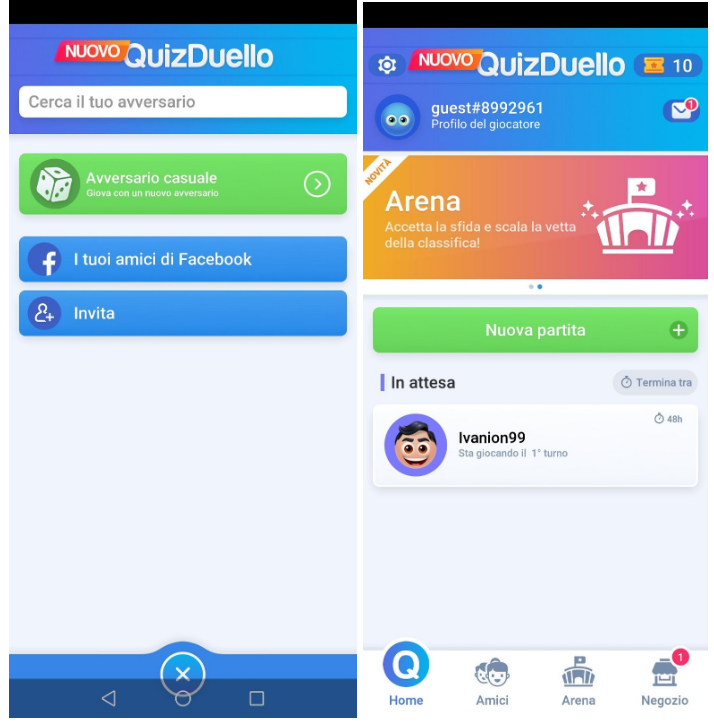
\includegraphics[width=1 \textwidth]{Figure22.png}
\caption{QuizDuello - Schermata principale e schermata degli amici}
\end{center}
\end{figure}

\begin{figure}[htp]
\begin{center}
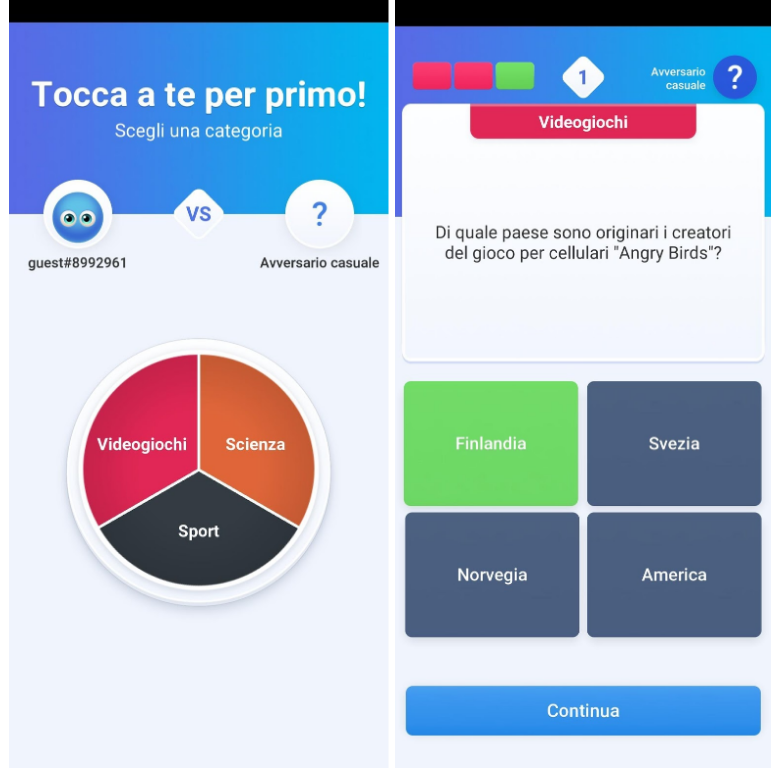
\includegraphics[width=1 \textwidth]{Figure23.png}
\caption{QuizDuello - Selezione della categoria delle domande e struttura delle domande}
\end{center}
\end{figure}

\begin{figure}[htp]
\begin{center}
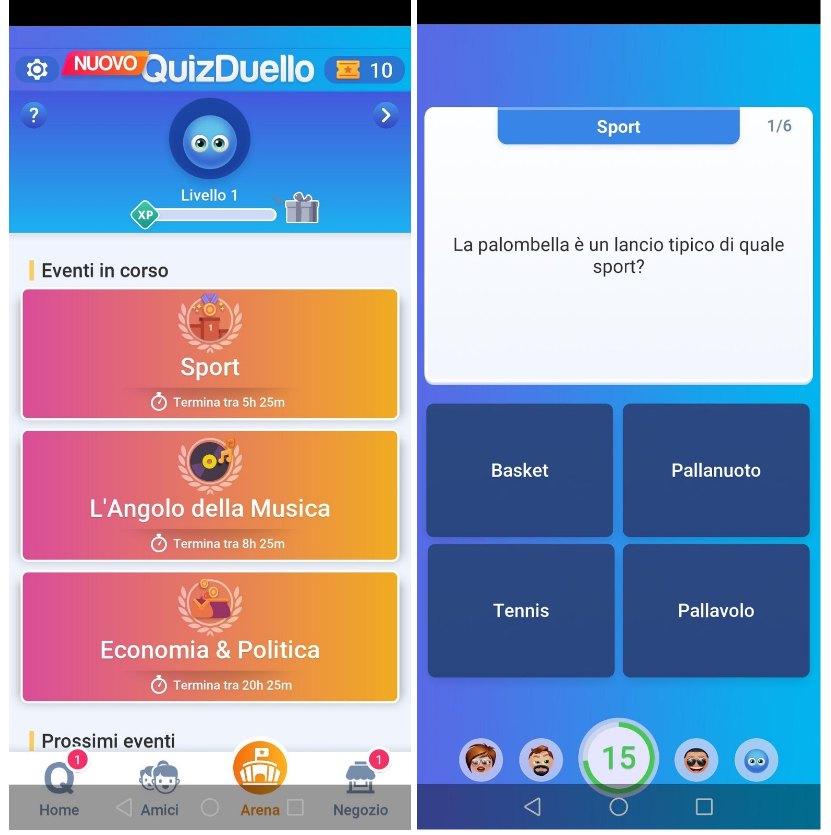
\includegraphics[width=1 \textwidth]{Figure24.png}
\caption{QuizDuello - Pagina eventi, struttura delle domande e classifica totale evento}
\end{center}
\end{figure}

\begin{figure}[htp]
\begin{center}
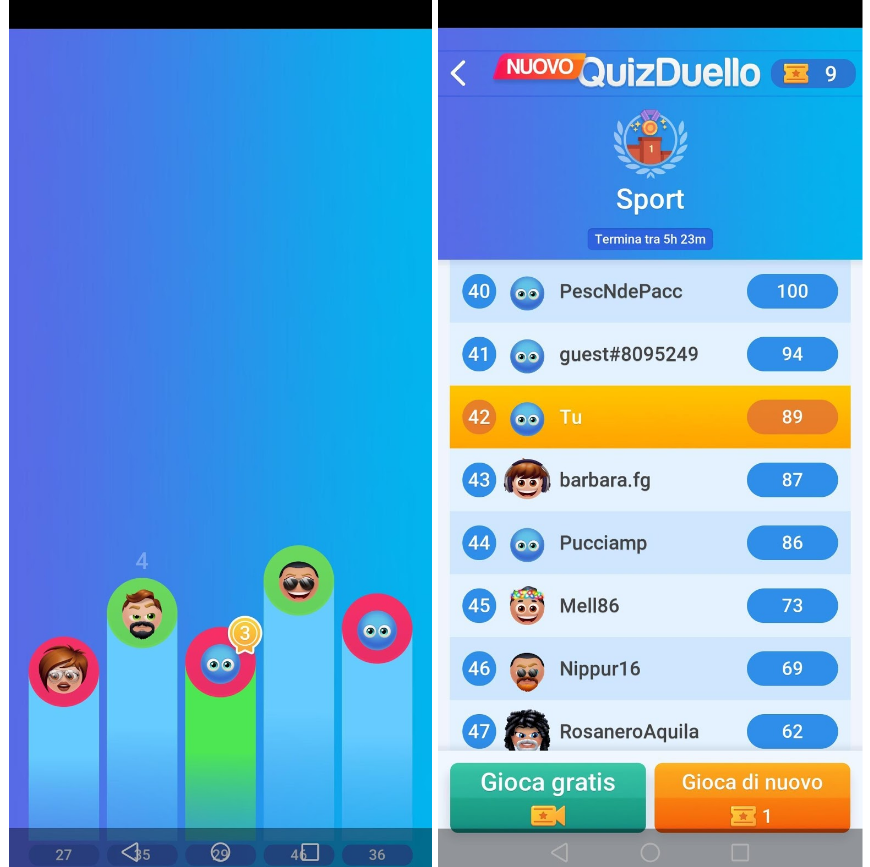
\includegraphics[width=1 \textwidth]{Figure25.png}
\caption{QuizDuello - Classifica totale evento}
\end{center}
\end{figure}


\end{document}